\section{Native readouts and a typed uniform observation map}\label{sec:uniform}
\subsection{State, clock and geometric registration}
Write the native state as $\Omega=x+iy\in\C^3$, with $x,y\in\R^3$. The sourced recurrence first forms
\begin{equation}\label{eq:native}
\widetilde\Omega_i=\Omega_i+\epsilon\Omega_i(k_i-|\Omega_i|^2)
+g(L_3\Omega)_i,\qquad
L_3=\begin{pmatrix}-2&1&1\\1&-2&1\\1&1&-2\end{pmatrix},
\end{equation}
then synchronizes phases simultaneously. If $\vartheta_i=\operatorname{Arg}_0\widetilde\Omega_i$, with $\operatorname{Arg}_0(0)=0$, its mathematical expression is
\begin{equation}\label{eq:sync}
\Omega_i^+=|\widetilde\Omega_i|\exp\!\left(i\left[\vartheta_i+\lambda_s
\sum_{j\ne i}\sin3(\vartheta_j-\vartheta_i)\right]\right).
\end{equation}
Exact zero components remain zero. The source's zero-strength branch returns the pre-sync state directly. These formulas identify the native object; we do not execute it or assert a physical time step. The shell, receiver positions and observation laws below are not arguments of the recurrence.~\cite{Native}

The separate face decoder assigns $D_i(\Omega_i)=x_i t_i+y_i\ez$ to the tangent plane of face $i$, with its sourced horizontal unit tangent $t_i$. This is a triple of face-attached vectors, not a single ambient vector at all exterior sites. Its area triple is the channel-indexed cross product below; the distinction motivates the explicit dictionary rather than an implicit conversion to a spatial field.~\cite{Native}

The staged readout uses a supplied clock $(q,N,t_c)$, where $q$ is integer, $N$ is a positive integer and $t_c$ is an independent scalar. Define
\begin{equation}\label{eq:staged}
\begin{aligned}
\kappa&=\norm{\Omega},& I&=\kappa^2,&\Ch&=x\times y,\\
\theta&=2\pi(q\bmod N)/N,&
b&=\lambda_{vp}e^{-\gamma t_c}\cos3(\theta-\ell),\\
z_s&=b\frac{\kappa}{1+\kappa},&
M&=z_s(\cos\theta,\sin\theta,1),&T&=\alpha M+\beta\Ch.
\end{aligned}
\end{equation}
The literal defaults are $(\lambda_{vp},\gamma,\ell,\alpha,\beta)=(0.618,0.577,0.244,1,0.5)$. We write $z_s$ for the sources' scalar $z$, avoiding confusion with a spatial coordinate. The observer index $k$ does not replace $q$. A changed clock can change $M$ at fixed $\Omega$, without any motion of an observer or native evolution.~\cite{Readout}

\begin{definition}[Conditional virtual dictionary]\label{def:dictionary}
Fix, before comparing states, $A=\lambda_gR_z(\delta)$ with $\lambda_g>0$. For each ordered readout triple $v\in\{M,\Ch,T\}$, define $W_v=Av$ as a virtual polar measurement vector. For a complete observer frame, a paired normal, and a circle tangent respectively, record
\begin{equation}\label{eq:uniform}
\begin{aligned}
y_k^v&=B_k\tr W_v,\qquad \mathcal R_k=(z_s,y_k^M,y_k^{\Ch},y_k^T),\\
g_j^\pm(v)&=(n_j^\pm)\tr W_v,\\
l_j(\chi;v)&=(-\sin\chi\,u_j+\cos\chi\,\ez)\tr W_v.
\end{aligned}
\end{equation}
\end{definition}
This is the uniform convention of SRG-03.~\cite[Eqns.~(3)--(6)]{SRG03} It maps labelled numerical data to linear measurement functionals. In particular $\Ch$ is not silently promoted to an ambient axial vector; $A$ is not asserted to intertwine native channel symmetries and spatial symmetries. A different physical typing would require a new dictionary, including the parity of any blend with $M$. The optional fixed calibration used for the accepted state-contrast figure is $\lambda_g=a$, $\delta=\pi/2-0.244$. No parameter is estimated from the contrasted states.

The components are taken in an orthonormal frame and are not divided by miniature scale. Distances and scales do not occur in \eqref{eq:uniform}; moving or resizing a module while preserving its frame cannot change these records. This is a declared uniform comparator. Under a passive orthogonal coordinate change $U$, transform $A$ to $UA$, $B_k$ to $UB_k$, and normals and tangents by $U$. Then $(UB_k)\tr(UA)v=B_k\tr Av$, so every record is unchanged. This includes reflected viewing coordinates. It does not claim invariance under active changes of native channels.

\subsection{Reconstruction, harmonics and paired redundancy}
\begin{theorem}[Uniform reconstruction]\label{thm:reconstruct}
For one registered $W=(W_x,W_y,W_z)$ and twelve frames at $\phi_k=\phi_0+2\pi k/12$,
\begin{equation}\label{eq:components}
y_k=(W_x\cos\phi_k+W_y\sin\phi_k,\ W_z,\ W_x\sin\phi_k-W_y\cos\phi_k).
\end{equation}
If $H$ stacks the $B_k\tr$, then
\begin{equation}\label{eq:gram}
H\tr H=12\Id_3,\quad \rank H=3,\quad
W=\frac1{12}\sum_{k=0}^{11}B_k y_k.
\end{equation}
The first and third component sequences contain only discrete spatial modes $\pm1$; the second is constant. There are 33 linear constraints on the 36 entries. For $L$ complete labelled rings the same statements hold with $12L$ replacing $12$.
\end{theorem}
\begin{proof}
The columns in \eqref{eq:frames} give \eqref{eq:components} directly. Each $B_kB_k\tr=\Id_3$, so summing gives the Gram identity. It is positive definite, proving rank three and the reconstruction formula. Rank-nullity gives codimension $36-3=33$ of the output range. Euler's identities express sine and cosine as combinations of $e^{\pm i\phi_k}$, proving the spatial support. At the opposite site $k+6$ the record is $(-y_{k,1},y_{k,2},-y_{k,3})$, and at $k+3$ it is $(-y_{k,3},y_{k,2},y_{k,1})$, by addition formulas. Summing over $12L$ orthonormal frames proves the extension, even if some labelled frames coincide between layouts.
\end{proof}
Already one complete known frame is invertible. Twelve frames provide redundant directional records and can test a convention; this calculation neither selects twelve as a physical number nor creates twelve independent source vectors. The angular index in the harmonic statement is spatial, not time.

\begin{proposition}[Paired-normal and tangent information]\label{prop:pairinfo}
Let $N_\Delta$ have the six rows $(n_j^\sigma)\tr$. Then
\begin{equation}\label{eq:patchgram}
G:=N_\Delta\tr N_\Delta=\diag(12/7,12/7,18/7),\qquad \rank N_\Delta=3,
\end{equation}
and
\begin{equation}\label{eq:pairinfo}
g_j^++g_j^-=\frac4{\sqrt7}u_j\cdot W,\qquad
g_j^+-g_j^-=\frac{2\sqrt3}{\sqrt7}W_z.
\end{equation}
All three differences agree; the three sums add to zero. A single pair misses exactly the direction $v_j$. At the circle contacts, $l_j^+=-g_j^+$ and $l_j^-=g_j^-$.
\end{proposition}
\begin{proof}
For one pair, summing $n n\tr$ cancels the mixed terms and gives $(8/7)u_ju_j\tr+(6/7)\ez\ez\tr$. The identities $\sum_j u_j=0$ and $\sum_j u_ju_j\tr=(3/2)\diag(1,1,0)$ yield \eqref{eq:patchgram}. Adding and subtracting the two normal projections gives \eqref{eq:pairinfo}; its constraints follow. The normals span the median plane, so their joint nullspace is $\R v_j$. The contact tangent signs are those of Theorem~\ref{thm:circle}. Thus the tangent values add no information beyond the normal readings in this uniform model.
\end{proof}
These are projections of $W$, not the derivatives of a macro trajectory. A nonzero $n\cdot M$ is not a crossing velocity; Section~\ref{sec:grazing} supplies an explicit distinction.

\section{What the staged observations retain about the state}\label{sec:rank}
For known $b\ne0$ and finite $\kappa\ge0$, the scalar relation in \eqref{eq:staged} is exactly invertible on $0\le z_s/b<1$:
\begin{equation}\label{eq:inverse}
\kappa=\frac{z_s}{b-z_s}.
\end{equation}
Known invertible $A$ and a complete frame recover $\Ch$. Hence the complete staged records are equivalent, as noiseless information, to $(I,\Ch)$. $M$ is fixed by $z_s$ and the clock, and $T$ is a blend of known terms. If only $z_s$ and $T$ are available, the additional hypothesis $\beta\ne0$ permits $\Ch=(T-\alpha M)/\beta$. $T$ alone need not separate its two contributions.

\begin{theorem}[Generic instantaneous native rank]\label{thm:rankfour}
Assume a fixed known clock and configuration with $b\ne0$, known $A$ with $\lambda_g>0$, and complete noiseless staged records including $\Ch$. On
\begin{equation}\label{eq:regular}
\Ch=x\times y\ne0,\qquad I=|x|^2+|y|^2>2\norm{\Ch},
\end{equation}
the map from the six real state coordinates to the records has rank four. Its local fibres have dimension two. Two independent invisible tangent directions are
\begin{equation}\label{eq:invisible}
U=(-y,x),\qquad V=(\Ch\times x,\Ch\times y).
\end{equation}
\end{theorem}
\begin{proof}
On the domain \eqref{eq:regular}, $I>0$ and $z_s=b\sqrt I/(1+\sqrt I)$ has nonzero derivative $b/[2\sqrt I(1+\sqrt I)^2]$. The preceding inverses reduce the rank calculation to the polynomial map $\Phi(x,y)=(I,x\times y)$. Its differential is
\[
dI=2x\cdot dx+2y\cdot dy,\qquad
d\Ch=dx\times y+x\times dy.
\]
A dependence with scalar coefficient $h$ and vector coefficient $d$ among its four rows would require
\begin{equation}\label{eq:rowdepend}
2h x+y\times d=0,\qquad 2h y+d\times x=0.
\end{equation}
Dotting the first equation with $x$ and the second with $y$, then subtracting, gives $h(|x|^2-|y|^2)=0$. Dotting with the other vector gives $h(x\cdot y)=0$. But
\[
I^2-4\norm{\Ch}^2=(|x|^2-|y|^2)^2+4(x\cdot y)^2>0.
\]
Therefore $h=0$. As $x,y$ are independent, $y\times d=d\times x=0$ forces $d=0$. The four rows are independent, establishing rank four throughout this open domain. The constant-rank theorem then gives two-dimensional local fibres.

For $U$, $dI=0$ and $d\Ch=(-y)\times y+x\times x=0$. For $V$, scalar products with the corresponding cross products vanish, while simultaneous infinitesimal rotation sends $\Ch$ to $\Ch\times\Ch=0$. Explicitly, $|U|^2=I$, $|V|^2=\norm{\Ch}^2I$ and $U\cdot V=-2\norm{\Ch}^2$. Their Gram determinant is $\norm{\Ch}^2(I^2-4\norm{\Ch}^2)>0$. They are independent and span the two-dimensional kernel.
\end{proof}

The first direction is common phase: $\Omega\mapsto e^{i\eta}\Omega$ preserves $I$ and $\Ch$. The second is a simultaneous real rotation of $x,y$ about their fixed cross-product axis. These are observation invariances. They do not assert that every such transformation is a symmetry of the native recurrence, especially at its phase convention for zero components. Rank four is a local statement, not a count of physical dimensions or a global uniqueness result.

\begin{proposition}[Exceptional strata and conditioning]\label{prop:singular}
For the polynomial map $\Phi=(I,\Ch)$, the rank is three at nonzero collinear $(x,y)$ and at maximal chirality $I=2\norm{\Ch}>0$, and zero at $(0,0)$. If $b=0$, the staged scalar and macro vector vanish; the remaining $\Ch$ map has rank three when $x,y$ are independent, two at a nonzero collinear pair, and zero at the origin. For $b\ne0$, the raw norm-based scalar is nondifferentiable at the origin.
\end{proposition}
\begin{proof}
A common phase is an invertible rotation of the pair $(x,y)$ leaving $\Phi$ unchanged. At a nonzero collinear pair it can arrange $y=0$, $x\ne0$. Then $dI=2x\cdot dx$ has rank one in $dx$, while $d\Ch=x\times dy$ has rank two in the independent $dy$ variables. This proves rank three for $\Phi$ and rank two for chirality alone.

Equality $I=2\norm{\Ch}>0$ in the displayed identity of the previous proof requires $|x|=|y|=r>0$ and $x\cdot y=0$. A proper spatial rotation gives $x=r e_1$, $y=r e_2$. In these coordinates
\[
d\Ch=(-r\,dx_3,-r\,dy_3,r(dx_1+dy_2)),\qquad
dI=2r(dx_1+dy_2).
\]
There are exactly three independent rows. For independent general $x,y$, a row dependence for chirality alone is \eqref{eq:rowdepend} with $h=0$, forcing $d=0$ and proving rank three. At the origin all polynomial first derivatives vanish. In contrast, along a nonzero real six-vector $v$, the staged scalar at $\varepsilon v$ is $b|\varepsilon|\norm v/(1+|\varepsilon|\norm v)$; its one-sided derivatives disagree when $b\ne0$.
\end{proof}

Exact inversion also has a conditioning cost. At fixed $b$, $\partial\kappa/\partial z_s=b/(b-z_s)^2=(1+\kappa)^2/b$. At fixed $z_s$, $\partial\kappa/\partial b=-z_s/(b-z_s)^2$. Thus saturation and a small nonzero clock coefficient amplify error. A clock zero is a mathematical blind setting; it is not claimed to occur on the literal default twelve-sector grid. Likewise a floating-point underflow or a rounded saturated value is not an exact zero or a finite invertible value. These mathematical statements retain the guarded numerical domains of the source without re-executing them.

\begin{figure}[htbp]\centering
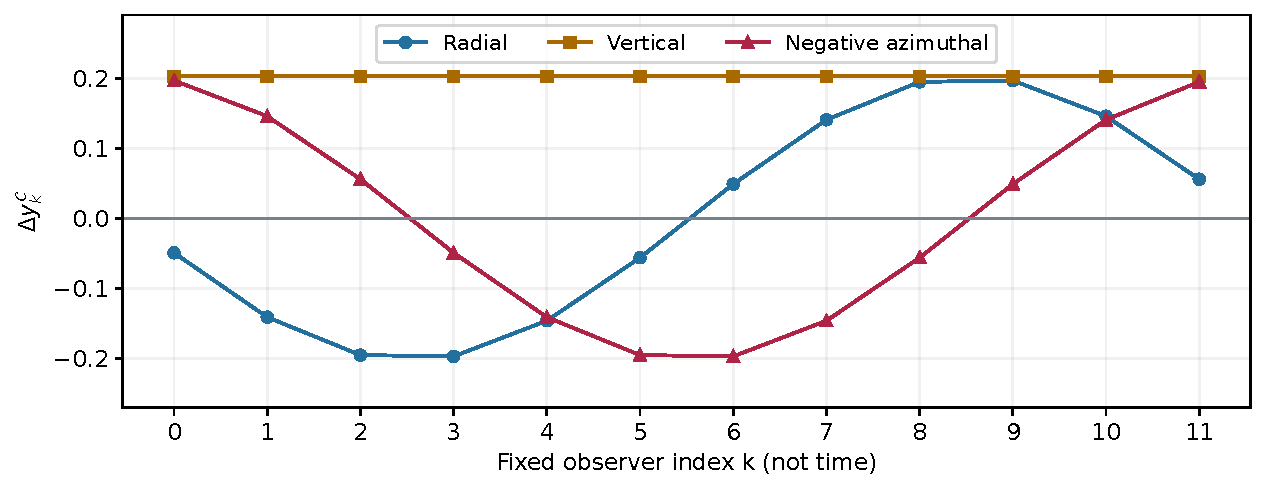
\includegraphics[width=\linewidth]{figures/state_contrast.pdf}
\caption{A fixed-state contrast from SRG-03: $(1,1,1)$ and $(1,e^{i\pi/6},1)$ have $I=3$, hence equal staged $z_s$ and $M$ at the common clock $(q,N,t_c)=(0,12,0)$. Chirality changes by $(-1/2,0,1/2)$. The plotted differences are $B_k\tr A\Delta\Ch$, using $A=aR_z(\pi/2-0.244)$ and $\phi_0=0$. They are fixed-site components with DC/first spatial harmonics, not successive native states or travelling data.}\label{fig:contrast}
\end{figure}

\section{A short cubic-information and subsystem comparison}\label{sec:cubic}
The historical handoff uses $J(\Omega)=\Im(\Omega_1\overline\Omega_2\Omega_3)$, which is not among the staged invariants. This limited comparison explains an information boundary without adopting a receiver model.

\begin{proposition}[Missing cubic data]\label{prop:cubic}
The complete uniform staged records, including every paired and circle-tangent projection, do not determine $J$. Consequently they do not determine the sourced historical parameter handoff from an arbitrary finite completed $J$ record.
\end{proposition}
\begin{proof}
Let $\Omega=(1,e^{i\pi/6},1)$ and $\Omega'=-\Omega$. Both have $I=3$ and $\Ch=(-1/2,0,1/2)$, so all staged records at a common clock coincide. But the cubic products are $e^{-i\pi/6}$ and $-e^{-i\pi/6}$, giving $J=-1/2$ and $J'=+1/2$. For a nonempty finite real record the handoff forms
\begin{equation}\label{eq:handoff}
\mathcal N=\frac{\operatorname{mean}|J|}{\max|J|},\quad
\mathcal S=\operatorname{sign}(\operatorname{mean}J_{\rm tail}),\quad
(\alpha_e,\mu_e,\gamma_e)=
(\alpha_0(0.3+0.7\mathcal N),\ 0.6+0.2\mathcal S,\ 0.1(1+\mathcal N)).
\end{equation}
The denominator is one for an all-zero record, and the tail is the last twenty entries only when there are more than twenty entries. In the two singleton records $\mathcal N=1$, but $\mu_e=0.4$ and $0.8$. Thus equal staged observations yield different handoff parameters. Missing or empty records have the separate fallback $(\alpha_0,0.6,0.2)$ and are not the all-zero case. Optional historical measurement noise is absent from this counterexample.~\cite{Historical,SRG03}
\end{proof}

One extra correctly aligned $J$ per retained row is sufficient to evaluate \eqref{eq:handoff}; the two final statistics plus a missing/empty flag suffice if only its final output is desired. A present value is not a history. This is a finite real, fixed-channel, fixed-phase convention: the old helper is not being given an unproved NaN/overflow contract. The already sourced EMA variant is a different observation family, so Proposition~\ref{prop:cubic} is not a theorem about every possible Z readout.

\subsection{The limited twelve-site comparison}
The recovered RSB array has indices in $\C^3\otimes\C^{12}\otimes\C^2$. One can conditionally assign its middle index to the twelve spatial sites, provided an origin/cut and internal basis are declared. Its internal channel and helicity labels are not thereby native faces, gap pairs or physical helicity. The periodic difference operator $(L_{12}f)_k=f_{k-1}+f_{k+1}-2f_k$ obeys
\begin{equation}\label{eq:laplacian}
L_{12}\mathbf1=0,\qquad
L_{12}\cos\phi=(\sqrt3-2)\cos\phi,\qquad
L_{12}\sin\phi=(\sqrt3-2)\sin\phi.
\end{equation}
Indeed substituting $e^{im\phi_k}$ gives multiplier $2\cos(2\pi m/12)-2$; set $m=0,\pm1$. This is algebraic compatibility of the observed spatial modes, not a continuum Laplacian with a recovered geometric radius factor. Site-independent linear channel/helicity maps preserve this support because they commute with the spatial Fourier decomposition.

The source contraction has a separate obstruction. It chooses the first index maximizing site intensity and, for active nonadaptive $0<\alpha_e\le1$, retains multiplier one there and $1-\alpha_e$ elsewhere. Constant nonzero site data are invariant under cyclic shifts, yet first-index tie selection gives a nonuniform output distinguished at site zero. Shifting this output changes it, whereas shifting the input does not. Thus the rule is not globally cyclic-equivariant on ties. Subsequent scalar normalization cannot remove the unequal multipliers. Zero contraction is a distinct case. This exact counterexample is sufficient for the site-assignment qualification; no rule is repaired or executed.~\cite{RSB,SRG03}

The historical caller selects parameters from a completed record before a separate receiver run. There is no recovered operator coupling \eqref{eq:uniform} continuously into that receiver, no assignment of its state to the local circle, and no return term to \eqref{eq:native}. The comparison retains the accepted information boundary rather than choosing an autonomous spectral subsystem as physical toroidal dynamics.
